%\VignetteIndexEntry{Years of life lost (YLL)}

\documentclass[a4paper,twoside,12pt]{report}

\newcommand{\Title}{Years of Life Lost (YLL)
  to disease\\Diabetes in DK as example}
\newcommand{\Tit}{YLL}
\newcommand{\Version}{February 1.2}
\newcommand{\Dates}{November 2017}
\newcommand{\Where}{SDC}
\newcommand{\Homepage}{\url{http://bendixcarstensen.com/Epi}}
\newcommand{\Faculty}{\begin{tabular}{rl}
Bendix Carstensen
  & Steno Diabetes Center, Gentofte, Denmark\\
  & {\small \& Department of Biostatistics,
               University of Copenhagen} \\
  & \texttt{b@bxc.dk}\\
  & \url{http://BendixCarstensen.com} \\[1em]
                      \end{tabular}}
%----------------------------------------------------------------------
% Packages
%\usepackage[inline]{showlabels}
%\usepackage[latin1]{inputenc}
\usepackage[utf8]{inputenc}
\usepackage[T1]{fontenc}
\usepackage[english]{babel}
\usepackage[font=it,labelfont=normalfont]{caption}
\usepackage[colorlinks,urlcolor=blue,linkcolor=red,citecolor=Maroon]{hyperref}
\usepackage[dvipsnames]{xcolor}
\usepackage[super]{nth}
% \usepackage[retainorgcmds]{IEEEtrantools}
\usepackage[noae]{Sweave}
\usepackage[ae,hyper]{Rd}
% \usepackage[noae]{C:/util/R/R-4.2.0/share/texmf/tex/latex/Sweave}
% \usepackage{C:/util/R/R-4.2.0/share/texmf/tex/latex/Rd}
\usepackage{makeidx,floatflt,amsmath,amsfonts,amsbsy,enumitem,dcolumn,needspace}
\usepackage{ifthen,calc,eso-pic,everyshi}
\usepackage{booktabs,longtable,rotating,graphicx,subfig}
\usepackage{pdfpages,verbatim,fancyhdr,datetime,afterpage}
\usepackage[abspath]{currfile}
% \usepackage{times}
\renewcommand{\textfraction}{0.0}
\renewcommand{\topfraction}{1.0}
\renewcommand{\bottomfraction}{1.0}
\renewcommand{\floatpagefraction}{0.9}
\definecolor{blaa}{RGB}{99,99,255}
\DeclareGraphicsExtensions{.png,.pdf,.jpg}
% Make the Sweave output nicer (slightly mor compact)
\DefineVerbatimEnvironment{Sinput}{Verbatim}{fontsize=\small,fontshape=sl,formatcom=\color{BlueViolet}}
\DefineVerbatimEnvironment{Soutput}{Verbatim}{fontsize=\small,formatcom=\color{Sepia},xleftmargin=0em}
\DefineVerbatimEnvironment{Scode}{Verbatim}{fontsize=\small}
\fvset{listparameters={\setlength{\topsep}{-0.1ex}}}
\renewenvironment{Schunk}%
{\renewcommand{\baselinestretch}{0.87} \vspace{\topsep}}%
{\renewcommand{\baselinestretch}{1.00} \vspace{\topsep}}
% \renewenvironment{knitrout}
% {\renewcommand{\baselinestretch}{0.87}}
% {\renewcommand{\baselinestretch}{1.00}}
% This is a file of useful extra commands snatched from
% Michael Hills, David Clayton, Bendix Carstensen & Esa Laara.
%

% Commands to draw observation lines on follow-up diagrams
%
% Horizontal lines
%
\providecommand{\hfail}[1]{\begin{picture}(250,5)
      \put(0,0){\line(1,0){#1}}
      \put(#1,0){\circle*{5}}
   \end{picture}}

\providecommand{\hcens}[1]{\begin{picture}(250,5)
      \put(0,0){\line(1,0){#1}}
      \put(#1,0){\line(0,1){2.5}}
      \put(#1,0){\line(0,-1){2.5}}
   \end{picture}}

%
% Diagonals for Lexis diagrams
%
\providecommand{\dfail}[1]{\begin{picture}(250,250)
      \put(0,0){\line(1,1){#1}}
      \put(#1,#1){\circle*{5}}
   \end{picture}}

\providecommand{\dcens}[1]{\begin{picture}(250,250)
      \put(0,0){\line(1,1){#1}}
%      \put(#1,#1){\line(0,1){2.5}}
%      \put(#1,#1){\line(0,-1){2.5}}
% BxC Changed this to an open circle instead of a line
      \put(#1,#1){\circle{5}}
   \end{picture}}

%
% Horizontal range diagrams
%
\providecommand{\hrange}[1]{\begin{picture}(200,5)
     \put(0,0){\circle*{5}}
     \put(0,0){\line(1,0){#1}}
     \put(0,0){\line(-1,0){#1}}
   \end{picture}}

%
% Tree drawing
%
\providecommand{\Tree}[3]{\setlength{\unitlength}{#1\unitlength}\begin{picture}(0,0)
   \put(0,0){\line(3, 2){1}}
   \put(0,0){\line(3,-2){1}}
   \put(0.81, 0.54){\makebox(0,0)[br]{\footnotesize #2\ }}
   \put(0.81,-0.54){\makebox(0,0)[tr]{\footnotesize #3\ }}
\end{picture}}

\providecommand{\Wtree}[3]{\setlength{\unitlength}{#1\unitlength}\begin{picture}(0,0)
   \put(0,0){\line(1, 1){1}}
   \put(0,0){\line(1,-1){1}}
   \put(0.8,0.8){\makebox(0,0)[br]{\footnotesize #2\ }}
   \put(0.8,-0.8){\makebox(0,0)[tr]{\footnotesize #3\ }}
\end{picture}}

\providecommand{\Ntree}[3]{\setlength{\unitlength}{#1\unitlength}\begin{picture}(0,0)
   \put(0,0){\line(2, 1){1}}
   \put(0,0){\line(2,-1){1}}
   \put(0.8,0.4){\makebox(0,0)[br]{\footnotesize #2\ }}
   \put(0.8,-0.4){\makebox(0,0)[tr]{\footnotesize #3\ }}
\end{picture}}

\providecommand{\Nutree}[3]{\setlength{\unitlength}{#1\unitlength}\begin{picture}(0,0)
   \put(0,0){\line(2, 1){#1}}
   \put(0,0){\line(2,-1){#1}}
   \put(0.8,0.4){\makebox(0,0)[br]{#2\ }}
   \put(0.8,-0.4){\makebox(0,0)[tr]{#3\ }}
\end{picture}}

%
% Tree drawing
%
\providecommand{\tree}[3]{\setlength{\unitlength}{#1}\begin{picture}(0,0)
   \put(0,0){\line(3,2){1}}
   \put(0,0){\line(3,-2){1}}
   \put(0.81,0.54){\makebox(0,0)[br]{\footnotesize #2\ }}
   \put(0.81,-0.54){\makebox(0,0)[tr]{\footnotesize #3\ }}
\end{picture}}

\providecommand{\wtree}[3]{\setlength{\unitlength}{#1}\begin{picture}(0,0)
   \put(0,0){\line(1,1){1}}
   \put(0,0){\line(1,-1){1}}
   \put(0.8,0.8){\makebox(0,0)[br]{\footnotesize #2\ }}
   \put(0.8,-0.8){\makebox(0,0)[tr]{\footnotesize #3\ }}
\end{picture}}

\providecommand{\ntree}[3]{\setlength{\unitlength}{#1}\begin{picture}(0,0)
   \put(0,0){\line(2,1){1}}
   \put(0,0){\line(2,-1){1}}
   \put(0.8,0.4){\makebox(0,0)[br]{\footnotesize #2\ }}
   \put(0.8,-0.4){\makebox(0,0)[tr]{\footnotesize #3\ }}
\end{picture}}

\providecommand{\nutree}[3]{\begin{picture}(0,0)
   \put(0,0){\line(2,1){#1}}
   \put(0,0){\line(2,-1){#1}}
   \put(0.8,0.4){\makebox(0,0)[br]{#2\ }}
   \put(0.8,-0.4){\makebox(0,0)[tr]{#3\ }}
\end{picture}}

%
% Other commands
%
\providecommand{\ip}[2]{\langle #1 \vert #2 \rangle} 
\providecommand{\I}{\text{\rm gI}}
\providecommand{\prob}[0]{\text{\rm Pr}}
\providecommand{\nhy}[0]{_{\oslash}}
\providecommand{\true}[0]{_{\text{\rm \tiny T}}}
\providecommand{\hyp}[0]{_{\text{\rm \tiny H}}}
% \providecommand{\mpydiv}[0]{\stackrel{\textstyle \times}{\div}}
% Changed to slightly smaller symbols
\providecommand{\mpydiv}[0]{\stackrel{\scriptstyle\times}{\scriptstyle\div}}
\providecommand{\mie}[1]{{\it #1}}
\providecommand{\mycircle}[0]{\circle*{5}}
\providecommand{\smcircle}[0]{\circle*{1}}
\providecommand{\corner}[0]{_{\text{\rm \tiny C}}}
\providecommand{\ind}[0]{\hspace{10pt}}
\providecommand{\gap}[0]{\\[5pt]}
\renewcommand{\S}[0]{section~}
\providecommand{\blank}[0]{$\;\,$}
\providecommand{\vone}{\vspace{1cm}}
\providecommand{\ljust}[1]{\multicolumn{1}{l}{#1}}
\providecommand{\cjust}[1]{\multicolumn{1}{c}{#1}}
\providecommand{\transpose}{^{\text{\sf T}}}
\providecommand{\histog}[5]{\rule{1mm}{#1mm}\,\rule{1mm}{#2mm}\,\rule{1mm}{#3mm}\,\rule{1mm}{#4mm}\,\rule{1mm}{#5mm}}
\providecommand{\pmiss}{P_{\mbox{\tiny miss}}}

% Below is BxCs commands inserted

% Only works with hyperref package:
\newcommand{\mailto}[1]{\href{mailto:#1}{\tt #1}}

\providecommand{\bc}{\begin{center}}
\providecommand{\ec}{\end{center}}
\providecommand{\bd}{\begin{description}}
\providecommand{\ed}{\end{description}}
\providecommand{\bi}{\begin{itemize}}
\providecommand{\ei}{\end{itemize}}
\providecommand{\bn}{\begin{equation}}
\providecommand{\en}{\end{equation}}
\providecommand{\be}{\begin{enumerate}}
\providecommand{\ee}{\end{enumerate}}
\providecommand{\bes}{\begin{eqnarray*}}
\providecommand{\ees}{\end{eqnarray*}}

\DeclareMathOperator{\Pp}{P}
\DeclareMathOperator{\pp}{p}
% \providecommand{\p}{{\mathrm p}}
\providecommand{\e}{{\mathrm e}}
\providecommand{\D}{{\mathrm D}}
\providecommand{\dif}{{\,\mathrm d}}
\providecommand{\pmat}[1]{\Pp\!\left\{#1\right\}}
\providecommand{\ptxt}[1]{\Pp\!\left\{\text{#1}\right\}}
\providecommand{\E}{\text{\rm E}}
\providecommand{\V}{\text{\rm V}}
\providecommand{\BLUP}{\text{\rm BLUP}}
\providecommand{\se}{\text{\rm s.e.}}
\providecommand{\sem}{\text{\rm s.e.m.}}
\providecommand{\std}{\text{\rm std}}
\providecommand{\sd}{\text{\rm s.d.}}
\providecommand{\Var}{\text{\rm var}}
\providecommand{\VAR}{\text{\rm var}}
\providecommand{\var}{\text{\rm var}}
\providecommand{\cov}{\text{\rm cov}}
\providecommand{\corr}{\text{\rm corr}}
\providecommand{\mean}{\text{\rm mean}}
\providecommand{\CV}{\text{\rm CV}}
\providecommand{\median}{\text{\rm median}}
\providecommand{\cv}{\text{\rm c.v.}}
\providecommand{\erf}{\text{\rm erf}}
\providecommand{\ef}{\text{\rm ef}}
\providecommand{\SSD}{\text{\rm SSD}}
\providecommand{\SPD}{\text{\rm SPD}}
\providecommand{\odds}{\text{\rm odds}}
\providecommand{\bin}{\text{\rm binom}}
\providecommand{\half}{\frac{1}{2}}
% \providecommand{\td}[0]{\stackrel{\textstyle \times}{\div}}
% Changed to slightly smaller symbols
\providecommand{\td}[0]{\stackrel{\scriptstyle \times}{\scriptstyle \div}}
\providecommand{\dt}[0]{\stackrel{\scriptstyle \div}{\scriptstyle \times}}
\providecommand{\diag}{\text{\rm diag}}
\providecommand{\det}{\text{\rm det}}
\providecommand{\dim}{\text{\rm dim}}
\providecommand{\spcol}{\text{\rm span}}
\providecommand{\logit}{\text{\rm logit}}
% \providecommand{\link}{\text{\rm link}}
\providecommand{\spn}{\text{\rm span}}
\providecommand{\CI}{\text{\rm CI}}
\providecommand{\IP}{\text{\rm IP}}
\providecommand{\OR}{\text{\rm OR}}
\providecommand{\RR}{\text{\rm RR}}
\providecommand{\ER}{\text{\rm ER}}
\providecommand{\EM}{\text{\rm EM}}
\providecommand{\EF}{\text{\rm EF}}
\providecommand{\RD}{\text{\rm RD}}
\providecommand{\AC}{\text{\rm AC}}
\providecommand{\AF}{\text{\rm AF}}
\providecommand{\PAF}{\text{\rm PAF}}
\providecommand{\AR}{\text{\rm AR}}
\providecommand{\CR}{\text{\rm CR}}
\providecommand{\PAR}{\text{\rm PAR}}
\providecommand{\EL}{\text{\rm EL}}
\providecommand{\ERL}{\text{\rm ERL}}
\providecommand{\YLL}{\text{\rm YLL}}
\providecommand{\SD}{\text{\rm SD}}
\providecommand{\SE}{\text{\rm SE}}
\providecommand{\SEM}{\text{\rm SEM}}
\providecommand{\SR}{\text{\rm SR}}
\providecommand{\SMR}{\text{\rm SMR}}
\providecommand{\RSR}{\text{\rm RSR}}
\providecommand{\CMF}{\text{\rm CMF}}
\providecommand{\pvp}{\text{\rm PV$+$}}
\providecommand{\pvn}{\text{\rm PV$-$}}
\providecommand{\R}{{\textsf{\textbf{R}}}}
\providecommand{\sas}{\textsl{\textbf{SAS}}}
\providecommand{\SAS}{\textsl{\textbf{SAS}}}
%\providecommand{\gap}[0]{\\[5pt]}
%\providecommand{\blank}[0]{$\;\,$}
% Conditional independence sign from Philip Dawid
\providecommand{\cip}{\mbox{$\perp\!\!\!\perp$}}

%%% Commands to comment out parts of the text
\providecommand{\GLEM}[1]{}
\providecommand{\FORGETIT}[1]{}
\providecommand{\OMIT}[1]{}

%%% Insert output from program in small text
%%% (requires package verbatim)
\providecommand{\insoutsmall}[1]{
% \small
 \footnotesize
 \renewcommand{\baselinestretch}{0.8}
 \verbatiminput{#1}
 \renewcommand{\baselinestretch}{1.0}
 \normalsize
}
\providecommand{\insout}[1]{
 \scriptsize
 \renewcommand{\baselinestretch}{0.8}
 \verbatiminput{#1}
 \renewcommand{\baselinestretch}{1.0}
 \normalsize
}
\providecommand{\insouttiny}[1]{
\tiny
\renewcommand{\baselinestretch}{0.8}
\verbatiminput{#1}
\renewcommand{\baselinestretch}{1.0}
\normalsize
}

% From Esa:
\providecommand{\T}{\text{\rm \small{T}}}
\providecommand{\id}{\text{\rm id}}
\providecommand{\Dev}{\text{\rm Dev}}
\providecommand{\Bin}{\text{\rm Bin}}
\providecommand{\probit}{\text{\rm probit}}
\providecommand{\cloglog}{\text{\rm cloglog}}

% Special commands to include output from R, Bugs and Stata

\providecommand{\Rin}[2]{
\subsection{\texttt{#1.R}}
#2

\insout{./R/#1.Rout}

}

\providecommand{\Statain}[2]{
\subsection{\texttt{#1.do}}
#2

\insout{./do/#1.log}

}

\providecommand{\Bugsin}[2]{
\subsection{\texttt{#1.bug}}
#2

\insout{./bugs/#1.bug}

}

\newlength{\wdth}
\providecommand{\fxbl}[1]{\settowidth{\wdth}{#1} \makebox[\wdth]{}}

%%% Local Variables:
%%% mode: latex
%%% TeX-master: t
%%% End:


%----------------------------------------------------------------------
% Set up layout of pages
\oddsidemargin 1mm
\evensidemargin 1mm
\topmargin -10mm
\headheight 8mm
\headsep 5mm
\textheight 240mm
\textwidth 165mm
%\footheight 5mm
\footskip 15mm
\renewcommand{\topfraction}{0.9}
\renewcommand{\bottomfraction}{0.9}
\renewcommand{\textfraction}{0.1}
\renewcommand{\floatpagefraction}{0.9}
\renewcommand{\headrulewidth}{0.1pt}
\setcounter{secnumdepth}{2}
\setcounter{tocdepth}{3}

%----------------------------------------------------------------------
% How to insert a figure in a .rnw file
\newcommand{\rwpre}{./graph/gr}
\newcommand{\insfig}[3]{
\begin{figure}[h]
  \centering
  \includegraphics[width=#2\textwidth]{\rwpre-#1}
% \caption{#3}
  \caption{#3\hfill\mbox{\footnotesize \textrm{\tt \rwpre-#1}}}
  \label{fig:#1}
% \afterpage{\clearpage}
\end{figure}}
\newcommand{\linput}[1]{
% \clearpage 
\afterpage{\hfill \ldots now input from \texttt{#1.tex}\\} 
\fancyfoot[OR,EL]{\footnotesize \texttt{#1.tex}} 
\input{#1}}

%----------------------------------------------------------------------
% Here is the document starting with the titlepage
\begin{document}

%----------------------------------------------------------------------
% The title page
\setcounter{page}{1}
\pagenumbering{roman}
\pagestyle{plain}
\thispagestyle{empty}
% \vspace*{0.05\textheight}
\flushright
% The blank below here is necessary in order not to muck up the
% linespacing in title if it has more than 2 lines
{\Huge \bfseries \Title

}\ \\[-1.5ex]
\noindent\textcolor{blaa}{\rule[-1ex]{\textwidth}{5pt}}\\[2.5ex]
\large
\Where \\
\Dates \\
\Homepage \\
\Version \\[1em]
\normalsize
Compiled \today,\ \currenttime\\
from: \texttt{\currfileabspath}\\[1em]
% \input{wordcount}
\normalsize
\vfill
\Faculty
% End of titlepage
\newpage

%----------------------------------------------------------------------
% Table of contents
\tableofcontents
% \listoftables
% \listoffigures
\clearpage
% \begingroup
% \let\clearpage\relax
% \listoftables
% \listoffigures
% \endgroup

%----------------------------------------------------------------------
% General text layout
\raggedright
\parindent 1em
\parskip 0ex
\cleardoublepage

%----------------------------------------------------------------------
% General page style
\pagenumbering{arabic}
\setcounter{page}{1}
\pagestyle{fancy}
\renewcommand{\chaptermark}[1]{\markboth{\textsl{#1}}{}}
\renewcommand{\sectionmark}[1]{\markright{\thesection\ \textsl{#1}}{}}
\fancyhead[EL]{\bf \thepage \quad \rm \rightmark}
\fancyhead[ER]{\rm \Tit}
\fancyhead[OL]{\rm \leftmark}
\fancyhead[OR]{\rm \rightmark \quad \bf \thepage}
\fancyfoot{}

\renewcommand{\rwpre}{./yll}

\chapter{Theory and technicalities}

This vignette for the \texttt{Epi} package describes the
probabilistic and demographic background for and technical implementation
of the \texttt{erl} and \texttt{yll} functions that computes the
expected residual life time and years of life lost in an illness-death
model.

\section{Years of life lost (YLL)}

\ldots to diabetes or any other disease for that matter.

The general concept in calculation of ``years lost to\ldots'' is the
comparison of the expected lifetime between two groups of persons; one
with and one without disease (in this example DM). The expected
lifetime is the area under the survival curve, so basically the
exercise requires that two survival curves that are deemed relevant be
available.

The years of life lost is therefore just the area between the survival
curves for those ``Well'', $S_W(t)$, and for those ``Diseased'',
$S_D(t)$:
\[
  \YLL = \int_0^\infty S_W(t) - S_D(t) \dif t
\]
The time $t$ could of course be age, but it could also be ``time after
age 50'' and the survival curves compared would then be survival
curves \emph{conditional} on survival till age 50, and the YLL would
be the years of life lost for a 50-year old person with diabetes.

If we are referring to the expected lifetime we will more precisely use
the label expected residual lifetime, ERL.

\section{Constructing the survival curves}

YLL can be computed in two different ways, depending on the way the
survival curve and hence the expected lifetime of a person
\emph{without} diabetes is computed:
\begin{itemize}
\item Assume that the ``Well'' persons are \emph{immune} to disease
  --- using only the non-DM mortality rates throughout for calculation
  of expected life time.
\item Assume that the ``Well'' persons \emph{can} acquire the disease and
  thereby see an increased mortality, thus involving all three rates
  shown in figure \ref{fig:states}.
\end{itemize}
The former gives a higher YLL because the comparison is to persons
assumed immune to DM (and yet with the same mortality as non-immune
prior to diagnosis), the latter gives a more realistic picture of the
comparison of group of persons with and without diabetes at a given
age that can be interpreted in the real world.

The differences can be illustrated by figure \ref{fig:states}; the
immune approach corresponds to an assumption of $\lambda(t)=0$ in the
calculation of the survival curve for a person in the ``Well'' state.

Calculation of the survival of a diseased person already in the ``DM''
state is unaffected by assumptions about $\lambda$.

\insfig{states}{0.7}{Illness-death model describing diabetes incidence
  and -mortality.}

\subsection{Total mortality --- a shortcut?}

A practical crude shortcut could be to compare the ERL in the diabetic
population to the ERL for the \emph{entire} population (that is use
the total mortality ignoring diabetes status).

Note however that this approach also counts the mortality of persons
that acquired the disease earlier, thus making the comparison
population on average more ill than the population we aim at, namely
those well at a given time, which only then become more gradually ill. 

How large these effects are can however be empirically explored, as we
shall do later.

\subsection{Disease duration}

In the exposition above there is no explicit provision for the effect of
disease duration, but if we were able to devise mortality rates for
any combination of age and duration, this could be taken into account.

There are however severe limitations in this as we in principle would
want to have duration effects as long as the age-effects --- in
principle for all $(a,d)$ where $d\leq A$, where $A$ is the age at
which we condition. So even if we were only to compute ERL from
age, say, 40 we would still need duration effects up to 60 years
(namely to age 100).

The incorporation of duration effects is in principle trivial from a
computational point of view, but we would be forced to entertain
models predicting duration effects way beyond what is actually
observed disease duration in any practical case.

\subsection{Computing integrals}

The practical calculations of survival curves, ERL and YLL involves
calculation of (cumulative) integrals of rates and functions of these
as we shall see below. This is easy if we have a closed form
expression of the function, so its value may be computed at any time
point --- this will be the case if we model rates by smooth parametric
functions.

Computing the (cumulative) integral of a function is done as follows: 
\begin{itemize}
\item Compute the value of the function (mortality rate for example)
  at the midpoints of a sequence of narrow equidistant intervals ---
  for example one- or three month intervals of age, say.
\item Take the cumulative sum of these values multiplied by the
  interval length --- this will be a very close approximation to the
  cumulative integral evaluated at the end of each interval.
\item If the intervals are really small (like 1/100 year), the
  distinction between the value at the middle and at the end of each
  interval becomes irrelevant.
\end{itemize}
Note that in the above it is assumed that the rates are given in units
corresponding to the interval length --- or more precisely, as the
cumulative rates over the interval.

\section{Survival functions in the illness-death model}

The survival functions for persons in the ``Well'' state can be
computed under two fundamentally different scenarios, depending on
whether persons in the ``Well'' state are assumed to be immune to the
disease ($\lambda(a)=0$) or not.

\subsection{Immune approach}

In this case both survival functions for person in the two states are
the usual simple transformation of the cumulative mortality rates:
\[
 S_W(a) = \exp\left(-\int_0^a\!\!\mu_W(u) \dif u \right), \qquad
 S_D(a) = \exp\left(-\int_0^a\!\!\mu_D(u) \dif u \right)
\]

\subsubsection{Conditional survival functions}

If we want the \emph{conditional} survival functions given survival to
age $A$, say, they are just:
\[
 S_W(a|A) = S_W(a)/S_W(A), \qquad S_D(a|A) = S_D(a)/S_D(A)
\]

\subsection{Non-immune approach}

For a diseased person, the survival function in this states is the same
as above, but the survival function for a person without disease (at
age 0) is (see figure \ref{fig:states}):
\[
S(a) = \ptxt{Well}\!(a) + \ptxt{DM}\!(a)
\]
In the appendix of the paper \cite{Carstensen.2008c} is an indication
of how to compute the probability of being in any of the four states
shown in figure \ref{fig:states}, which I shall repeat here:

In terms of the rates, the probability of being in the ``Well'' box is
simply the probability of escaping both death (at a rate of $\mu_W(a)$)
and diabetes (at a rate of $\lambda(a)$):
\[  
   \ptxt{Well}(a)  = \exp\left(\!-\int_0^a\!\!\mu_W(u)+\lambda(u) \right) \dif u
\]
The probability of being alive with diabetes at age $a$, is computed given that
 diabetes occurred at age $s$ ($s<a$) and then integrated over $s$ from $0$
 to $a$:
\begin{align*}
 \ptxt{DM}(a) = \int_0^a\!\! & \ptxt{survive to $s$, DM diagnosed at $s$} \\
                & \times \ptxt{survive with DM from $s$ to $a$} \dif s \\
              = \int_0^a\!\! & \lambda(s) 
                           \exp\left(\!-\int_0^s\!\!\mu_W(u)+\lambda(u) \dif u \right) \\
                & \times \exp\left(\!-\int_s^a\!\!\mu_D(u) \dif u \right) \dif s
\end{align*}
Sometimes we will use a version where the mortality among diabetes
patients depend both on age $a$ and duration of diabetes, $d$,
$\mu_D(a,d)$, in which case we get:
\begin{align*}
 \ptxt{DM}(a) = \int_0^a \! & \lambda(s) 
                           \exp\left(-\int_0^s\!\mu_W(u)+\lambda(u) \dif u \right) \\
                & \times \exp\left(-\int_s^a\!\mu_D(u,u-s) \dif u \right) \dif s
\end{align*}
because the integration variable $u$ is the age-scale and the second
integral refers to mortality among persons diagnosed at age $s$, that
is, with duration $u-s$ at age $u$.

The option of using duration-dependent mortality rates among diseased
individuals is not implemented yet.

\subsubsection{Conditional survival functions}

Unlike the immune approach, the conditional survival function in the
more realistic case is not just a ratio of the unconditional to the
value at the conditioning age, $A$, say. This would amount to
conditioning on being merely \emph{alive} at age $A$, but what we want
is to condition on being in the ``Well'' state at age $A$.

The formulae for the conditional probabilities of being either in
``Well'' or ``DM'', given being in ``Well'' at age $A$ are basically
replicates of the unconditional, albeit with changes in integration
limits:
\begin{align*}
\ptxt{Well|Well at $A$}(a) &= \exp\left(-\int_A^a \! \mu_W(u)+\lambda(u) \right) \dif u \\
  \ptxt{DM|Well at $A$}(a) &= \int_A^a \! \lambda(s) 
                               \exp\left(-\int_A^s\!\mu_W(u)+\lambda(u) \dif u \right) \\
                           & \qquad \times \exp\left(-\int_s^a\!\mu_D(u,u-s) \dif u \right) \dif s
\end{align*}
The calculation of these conditional survival functions is implemented
but not allowing for duration-dependence. Thus it is only implemented
assuming $\mu_D(a,d)=\mu_D(a)$.

\chapter{Analyses for DM in Denmark}

The rates we use as basis for the following calculations are derived
from the NDR, where we have omitted the blood-glucose criteria,
because there is compelling evidence that these have quite a low
specificity (particularly in the younger ages among women), and do
not substantially contribute to the sensitivity.

As noted above the calculations of YLL requires access to
(age-specific) rates of incidence of DM and mortality for persons with
and without DM.

\section{Modeling mortality and incidence data}

We read in the dataset of DM and population mortality and incidence, \texttt{DMepi}:
\begin{Schunk}
\begin{Sinput}
> data( DMepi )
\end{Sinput}
\end{Schunk}
The dataset \texttt{DMepi} contains diabetes events, deaths and
person-years for persons without diabetes and deaths and person-years
for persons with diabetes:
\begin{Schunk}
\begin{Sinput}
> str( DMepi )
\end{Sinput}
\begin{Soutput}
'data.frame':	4200 obs. of  8 variables:
 $ sex : Factor w/ 2 levels "M","F": 1 1 1 1 1 1 1 1 1 1 ...
 $ A   : num  0 0 0 0 0 0 0 0 0 0 ...
 $ P   : num  1996 1997 1998 1999 2000 ...
 $ D.DM: num  0 0 0 0 0 0 0 0 0 0 ...
 $ Y.DM: num  0.484 0.64 1.641 0.552 2.507 ...
 $ X   : num  1 2 4 4 4 1 1 3 4 1 ...
 $ D.nD: num  28 19 20 11 21 16 21 15 16 16 ...
 $ Y.nD: num  35469 35085 34240 34056 34002 ...
\end{Soutput}
\begin{Sinput}
> head( DMepi )
\end{Sinput}
\begin{Soutput}
  sex A    P D.DM      Y.DM X D.nD     Y.nD
2   M 0 1996    0 0.4839151 1   28 35468.92
3   M 0 1997    0 0.6399726 2   19 35085.18
4   M 0 1998    0 1.6406571 4   20 34240.14
5   M 0 1999    0 0.5523614 4   11 34055.52
6   M 0 2000    0 2.5065024 4   21 34002.22
7   M 0 2001    0 0.1184120 1   16 34177.39
\end{Soutput}
\end{Schunk}
For each combination of sex, age, period and date of birth in 1 year
age groups, we have the person-years in the ``Well'' (\texttt{Y.nD})
and the ``DM'' (\texttt{Y.DM}) states, as well as the number of deaths
from these (\texttt{D.nD}, \texttt{D.DM}) and the number of incident
diabetes cases from the ``Well'' state (\texttt{X}).

In order to compute the years of life lost to diabetes and how this
has changed over time, we fit models for the mortality and incidence
of both groups (and of course, separately for men and women). The
models we use will be age-period-cohort models \cite{Carstensen.2007a}
providing estimated mortality rates for ages 0--99 and dates
1.1.1996--1.1.2016.

First we transform the age and period variables to reflect the mean
age and period in each of the Lexis triangles. We also compute the
total number of deaths and amount of risk time, as we are going to
model the total mortality as well. Finally we restrict the dataset to
ages over 30 only:
\begin{Schunk}
\begin{Sinput}
> DMepi <- transform( subset( DMepi, A>30 ),
+                     D.T = D.nD + D.DM, 
+                     Y.T = Y.nD + Y.DM )
> head(DMepi)
\end{Sinput}
\begin{Soutput}
    sex  A    P D.DM     Y.DM  X D.nD     Y.nD D.T      Y.T
684   M 31 1996    0 305.9671 29   51 44161.83  51 44467.80
685   M 31 1997    2 326.2074 31   54 45508.64  56 45834.85
686   M 31 1998    2 340.1759 34   46 44954.45  48 45294.63
687   M 31 1999    5 330.9918 24   39 41148.97  44 41479.96
688   M 31 2000    1 332.0876 41   26 39027.30  27 39359.39
689   M 31 2001    2 310.8467 35   33 37975.78  35 38286.63
\end{Soutput}
\end{Schunk}
With the correct age and period coding in the Lexis triangles, we fit
models for the mortalities and incidences. Note that we for
comparative purposes also fit a model for the \emph{total} mortality,
ignoring the 
\begin{Schunk}
\begin{Sinput}
> # Knots used in all models
> ( a.kn <- seq(40,95,,6) )
\end{Sinput}
\begin{Soutput}
[1] 40 51 62 73 84 95
\end{Soutput}
\begin{Sinput}
> ( p.kn <- seq(1997,2015,,4) )
\end{Sinput}
\begin{Soutput}
[1] 1997 2003 2009 2015
\end{Soutput}
\begin{Sinput}
> ( c.kn <- seq(1910,1976,,6) )
\end{Sinput}
\begin{Soutput}
[1] 1910.0 1923.2 1936.4 1949.6 1962.8 1976.0
\end{Soutput}
\begin{Sinput}
> # Check the number of events between knots
> ae <- xtabs( cbind(D.nD,D.DM,X) ~ cut(A,c(30,a.kn,Inf)) + sex, data=DMepi )
> ftable( addmargins(ae,1), col.vars=3:2 )
\end{Sinput}
\begin{Soutput}
                               D.nD          D.DM             X       
                         sex      M      F      M      F      M      F
cut(A, c(30, a.kn, Inf))                                              
(30,40]                        9135   4650    597    277  12080   9648
(40,51]                       25535  15784   2947   1439  35445  23925
(51,62]                       59698  40171  10838   5253  60539  40034
(62,73]                      106519  81253  26197  14299  55908  44221
(73,84]                      158365 156678  34510  28834  27985  30381
(84,95]                      100880 179466  16194  25317   5272   8967
(95,Inf]                       6095  21414    640   1928     90    288
Sum                          466227 499416  91923  77347 197319 157464
\end{Soutput}
\begin{Sinput}
> pe <- xtabs( cbind(D.nD,D.DM,X) ~ cut(P,c(1990,p.kn,Inf)) + sex, data=DMepi )
> ftable( addmargins(pe,1), col.vars=3:2 )
\end{Sinput}
\begin{Soutput}
                                 D.nD          D.DM             X       
                           sex      M      F      M      F      M      F
cut(P, c(1990, p.kn, Inf))                                              
(1990,1997]                     51569  53567   6407   5990  13175  10960
(1997,2003]                    144136 155695  22390  19922  49805  41277
(2003,2009]                    131159 141782  26079  22249  60554  48066
(2009,2015]                    119812 127714  31285  24704  63440  49457
(2015,Inf]                      19551  20658   5762   4482  10345   7704
Sum                            466227 499416  91923  77347 197319 157464
\end{Soutput}
\begin{Sinput}
> ce <- xtabs( cbind(D.nD,D.DM,X) ~ cut(P-A,c(-Inf,c.kn,Inf)) + sex, data=DMepi )
> ftable( addmargins(ce,1), col.vars=3:2 )
\end{Sinput}
\begin{Soutput}
                                     D.nD          D.DM             X       
                               sex      M      F      M      F      M      F
cut(P - A, c(-Inf, c.kn, Inf))                                              
(-Inf,1.91e+03]                     19679  49020   2004   4446    599   1416
(1.91e+03,1.92e+03]                129799 189192  19780  26870  10665  15275
(1.92e+03,1.94e+03]                158953 152454  35667  28471  37850  36659
(1.94e+03,1.95e+03]                 99058  72432  25494  13074  71489  50631
(1.95e+03,1.96e+03]                 44129  28315   7534   3731  51750  34255
(1.96e+03,1.98e+03]                 13598   7484   1373    720  22942  17689
(1.98e+03, Inf]                      1011    519     71     35   2024   1539
Sum                                466227 499416  91923  77347 197319 157464
\end{Soutput}
\begin{Sinput}
> # Fit an APC-model for all transitions, seperately for men and women
> mW.m <- glm( D.nD ~ -1 + Ns(A  ,knots=a.kn,int=TRUE) +
+                          Ns(  P,knots=p.kn,ref=2005) +
+                          Ns(P-A,knots=c.kn,ref=1950), 
+            offset = log(Y.nD),
+            family = poisson,
+              data = subset( DMepi, sex=="M" ) )
> mD.m <- update( mW.m,  D.DM ~ . , offset=log(Y.DM) )
> mT.m <- update( mW.m,  D.T  ~ . , offset=log(Y.T ) )
> lW.m <- update( mW.m,  X ~ . )
> # Model for women
> mW.f <- update( mW.m, data = subset( DMepi, sex=="F" ) )
> mD.f <- update( mD.m, data = subset( DMepi, sex=="F" ) )
> mT.f <- update( mT.m, data = subset( DMepi, sex=="F" ) )
> lW.f <- update( lW.m, data = subset( DMepi, sex=="F" ) )
\end{Sinput}
\end{Schunk}

\section{Residual life time and years lost to DM}

We now collect the estimated years of life lost classified by method
(immune assumption or not), sex, age and calendar time:
\begin{Schunk}
\begin{Sinput}
> a.ref <- 30:90
> p.ref <- 1996:2016
> aYLL <- NArray( list( type = c("Imm","Tot","Sus"),
+                        sex = levels( DMepi$sex ),
+                        age = a.ref,
+                       date = p.ref ) )
> str( aYLL )
\end{Sinput}
\begin{Soutput}
 logi [1:3, 1:2, 1:61, 1:21] NA NA NA NA NA NA ...
 - attr(*, "dimnames")=List of 4
  ..$ type: chr [1:3] "Imm" "Tot" "Sus"
  ..$ sex : chr [1:2] "M" "F"
  ..$ age : chr [1:61] "30" "31" "32" "33" ...
  ..$ date: chr [1:21] "1996" "1997" "1998" "1999" ...
\end{Soutput}
\begin{Sinput}
> system.time(
+ for( ip in p.ref )
+    {
+    nd <- data.frame( A = seq(30,90,0.2)+0.1,
+                      P = ip,
+                   Y.nD = 1,
+                   Y.DM = 1,
+                   Y.T  = 1 )
+    muW.m <- ci.pred( mW.m, nd )[,1]
+    muD.m <- ci.pred( mD.m, nd )[,1]
+    muT.m <- ci.pred( mT.m, nd )[,1]
+    lam.m <- ci.pred( lW.m, nd )[,1]
+    muW.f <- ci.pred( mW.f, nd )[,1]
+    muD.f <- ci.pred( mD.f, nd )[,1]
+    muT.f <- ci.pred( mT.f, nd )[,1]
+    lam.f <- ci.pred( lW.f, nd )[,1]
+    aYLL["Imm","M",,paste(ip)] <- yll( int=0.2, muW.m, muD.m, lam=NULL, 
+                                       A=a.ref, age.in=30, note=FALSE )[-1]
+    aYLL["Imm","F",,paste(ip)] <- yll( int=0.2, muW.f, muD.f, lam=NULL,  
+                                       A=a.ref, age.in=30, note=FALSE )[-1]
+    aYLL["Tot","M",,paste(ip)] <- yll( int=0.2, muT.m, muD.m, lam=NULL,  
+                                       A=a.ref, age.in=30, note=FALSE )[-1]
+    aYLL["Tot","F",,paste(ip)] <- yll( int=0.2, muT.f, muD.f, lam=NULL,  
+                                       A=a.ref, age.in=30, note=FALSE )[-1]
+    aYLL["Sus","M",,paste(ip)] <- yll( int=0.2, muW.m, muD.m, lam=lam.m, 
+                                       A=a.ref, age.in=30, note=FALSE )[-1]
+    aYLL["Sus","F",,paste(ip)] <- yll( int=0.2, muW.f, muD.f, lam=lam.f, 
+                                       A=a.ref, age.in=30, note=FALSE )[-1]
+    } )
\end{Sinput}
\begin{Soutput}
   user  system elapsed 
 16.929   8.549  14.974 
\end{Soutput}
\begin{Sinput}
> round( ftable( aYLL[,,seq(1,61,10),], col.vars=c(3,2) ), 1 )
\end{Sinput}
\begin{Soutput}
          age   30        40        50        60        70        80        90     
          sex    M    F    M    F    M    F    M    F    M    F    M    F    M    F
type date                                                                          
Imm  1996     11.3 10.2  9.4  9.1  7.4  7.6  5.4  5.9  3.4  3.8  1.5  1.6  0.0  0.0
     1997     11.1  9.9  9.2  8.9  7.3  7.4  5.3  5.7  3.3  3.7  1.4  1.5  0.0  0.0
     1998     10.9  9.7  9.1  8.6  7.2  7.2  5.3  5.5  3.3  3.6  1.4  1.5  0.0  0.0
     1999     10.7  9.4  9.0  8.4  7.1  7.0  5.2  5.3  3.3  3.5  1.4  1.5  0.0  0.0
     2000     10.5  9.1  8.8  8.2  6.9  6.8  5.1  5.1  3.2  3.4  1.4  1.4  0.0  0.0
     2001     10.3  8.9  8.6  7.9  6.8  6.6  5.0  5.0  3.1  3.2  1.3  1.4  0.0  0.0
     2002     10.0  8.6  8.4  7.7  6.6  6.3  4.9  4.8  3.1  3.1  1.3  1.3  0.0  0.0
     2003      9.7  8.3  8.2  7.4  6.4  6.1  4.7  4.6  3.0  3.0  1.3  1.3  0.0  0.0
     2004      9.4  8.0  7.9  7.1  6.2  5.9  4.5  4.4  2.8  2.8  1.2  1.2  0.0  0.0
     2005      9.0  7.6  7.6  6.9  6.0  5.6  4.4  4.1  2.7  2.6  1.1  1.1  0.0  0.0
     2006      8.6  7.3  7.4  6.6  5.8  5.4  4.2  3.9  2.6  2.5  1.1  1.1  0.0  0.0
     2007      8.3  7.0  7.1  6.3  5.5  5.2  4.0  3.8  2.5  2.4  1.0  1.0  0.0  0.0
     2008      8.0  6.8  6.8  6.1  5.4  5.0  3.8  3.6  2.4  2.2  1.0  0.9  0.0  0.0
     2009      7.7  6.6  6.6  6.0  5.2  4.9  3.7  3.5  2.3  2.1  0.9  0.9  0.0  0.0
     2010      7.5  6.4  6.5  5.8  5.1  4.8  3.7  3.4  2.2  2.1  0.9  0.9  0.0  0.0
     2011      7.4  6.3  6.4  5.8  5.1  4.7  3.6  3.4  2.2  2.0  0.9  0.8  0.0  0.0
     2012      7.3  6.3  6.4  5.7  5.1  4.7  3.6  3.3  2.2  2.0  0.9  0.8  0.0  0.0
     2013      7.3  6.2  6.4  5.7  5.1  4.7  3.6  3.3  2.2  2.0  0.9  0.8  0.0  0.0
     2014      7.3  6.2  6.4  5.7  5.1  4.7  3.7  3.4  2.2  2.0  0.9  0.8  0.0  0.0
     2015      7.3  6.2  6.4  5.7  5.2  4.8  3.7  3.4  2.3  2.0  0.9  0.8  0.0  0.0
     2016      7.3  6.2  6.4  5.7  5.2  4.8  3.8  3.4  2.3  2.0  0.9  0.8  0.0  0.0
Tot  1996     10.7  9.8  8.8  8.7  6.9  7.2  5.0  5.5  3.1  3.5  1.3  1.4  0.0  0.0
     1997     10.5  9.5  8.6  8.4  6.7  7.0  4.9  5.3  3.0  3.4  1.3  1.4  0.0  0.0
     1998     10.3  9.2  8.5  8.2  6.6  6.8  4.8  5.1  3.0  3.3  1.3  1.4  0.0  0.0
     1999     10.0  8.9  8.3  7.9  6.5  6.5  4.7  4.9  2.9  3.2  1.3  1.3  0.0  0.0
     2000      9.8  8.7  8.1  7.7  6.3  6.3  4.6  4.7  2.9  3.1  1.2  1.3  0.0  0.0
     2001      9.6  8.4  7.9  7.4  6.2  6.1  4.5  4.6  2.8  2.9  1.2  1.2  0.0  0.0
     2002      9.3  8.1  7.7  7.2  6.0  5.9  4.3  4.4  2.7  2.8  1.2  1.2  0.0  0.0
     2003      9.0  7.8  7.5  6.9  5.8  5.6  4.2  4.2  2.6  2.7  1.1  1.1  0.0  0.0
     2004      8.6  7.5  7.2  6.6  5.6  5.4  4.0  4.0  2.5  2.5  1.1  1.1  0.0  0.0
     2005      8.3  7.1  6.9  6.4  5.3  5.1  3.8  3.7  2.4  2.4  1.0  1.0  0.0  0.0
     2006      7.9  6.8  6.6  6.1  5.1  4.9  3.6  3.6  2.2  2.2  0.9  0.9  0.0  0.0
     2007      7.6  6.5  6.4  5.9  4.9  4.7  3.4  3.4  2.1  2.1  0.9  0.9  0.0  0.0
     2008      7.3  6.3  6.1  5.6  4.7  4.5  3.3  3.2  2.0  2.0  0.8  0.8  0.0  0.0
     2009      7.0  6.1  5.9  5.5  4.5  4.4  3.2  3.1  1.9  1.9  0.8  0.8  0.0  0.0
     2010      6.8  5.9  5.8  5.4  4.4  4.3  3.1  3.0  1.8  1.8  0.8  0.7  0.0  0.0
     2011      6.7  5.8  5.7  5.3  4.4  4.3  3.0  3.0  1.8  1.7  0.7  0.7  0.0  0.0
     2012      6.6  5.8  5.6  5.2  4.3  4.2  3.0  2.9  1.8  1.7  0.7  0.7  0.0  0.0
     2013      6.5  5.7  5.6  5.2  4.3  4.2  3.0  2.9  1.8  1.7  0.7  0.7  0.0  0.0
     2014      6.5  5.7  5.6  5.2  4.4  4.2  3.0  2.9  1.8  1.7  0.7  0.7  0.0  0.0
     2015      6.4  5.6  5.6  5.2  4.4  4.2  3.1  2.9  1.8  1.7  0.7  0.7  0.0  0.0
     2016      6.4  5.6  5.6  5.2  4.4  4.3  3.1  3.0  1.8  1.7  0.8  0.7  0.0  0.0
Sus  1996     10.3  9.4  8.4  8.4  6.6  7.0  5.0  5.5  3.2  3.6  1.4  1.5  0.0  0.0
     1997     10.1  9.2  8.3  8.2  6.5  6.8  4.9  5.3  3.1  3.5  1.4  1.5  0.0  0.0
     1998      9.9  8.9  8.1  7.9  6.4  6.6  4.8  5.1  3.1  3.4  1.4  1.5  0.0  0.0
     1999      9.7  8.6  8.0  7.7  6.3  6.4  4.7  4.9  3.1  3.3  1.4  1.4  0.0  0.0
     2000      9.4  8.3  7.8  7.4  6.1  6.2  4.6  4.7  3.0  3.2  1.3  1.4  0.0  0.0
     2001      9.2  8.1  7.6  7.2  6.0  5.9  4.5  4.5  2.9  3.0  1.3  1.3  0.0  0.0
     2002      8.9  7.8  7.4  6.9  5.8  5.7  4.4  4.4  2.8  2.9  1.3  1.3  0.0  0.0
     2003      8.6  7.5  7.2  6.7  5.6  5.5  4.2  4.2  2.7  2.8  1.2  1.2  0.0  0.0
     2004      8.3  7.1  6.9  6.4  5.4  5.3  4.0  4.0  2.6  2.6  1.2  1.2  0.0  0.0
     2005      7.9  6.8  6.6  6.1  5.2  5.0  3.8  3.8  2.5  2.5  1.1  1.1  0.0  0.0
     2006      7.5  6.5  6.3  5.9  5.0  4.8  3.7  3.6  2.4  2.3  1.0  1.0  0.0  0.0
     2007      7.2  6.3  6.1  5.6  4.7  4.6  3.5  3.4  2.3  2.2  1.0  1.0  0.0  0.0
     2008      6.9  6.0  5.9  5.5  4.6  4.5  3.4  3.3  2.2  2.1  0.9  0.9  0.0  0.0
     2009      6.7  5.8  5.7  5.3  4.4  4.3  3.3  3.2  2.1  2.0  0.9  0.9  0.0  0.0
     2010      6.5  5.7  5.6  5.2  4.4  4.3  3.2  3.1  2.0  1.9  0.9  0.8  0.0  0.0
     2011      6.4  5.6  5.5  5.1  4.3  4.2  3.2  3.1  2.0  1.9  0.9  0.8  0.0  0.0
     2012      6.4  5.6  5.5  5.1  4.4  4.2  3.2  3.1  2.0  1.9  0.9  0.8  0.0  0.0
     2013      6.4  5.6  5.5  5.1  4.4  4.3  3.2  3.1  2.0  1.9  0.9  0.8  0.0  0.0
     2014      6.4  5.6  5.5  5.2  4.5  4.3  3.3  3.1  2.1  1.9  0.9  0.8  0.0  0.0
     2015      6.4  5.6  5.6  5.2  4.5  4.4  3.3  3.1  2.1  1.9  0.9  0.8  0.0  0.0
     2016      6.4  5.6  5.6  5.2  4.6  4.4  3.4  3.2  2.1  1.9  0.9  0.8  0.0  0.0
\end{Soutput}
\end{Schunk}
We now have the relevant points for the graph showing YLL to diabetes
for men and women by age, and calendar year, both under the immunity
and susceptibility models for the calculation of YLL.
\begin{Schunk}
\begin{Sinput}
> plyll <- function(wh){
+ par( mfrow=c(1,2), mar=c(3,3,1,1), mgp=c(3,1,0)/1.6, bty="n", las=1 )
+ 
+ matplot( a.ref, aYLL[wh,"M",,],
+          type="l", lty=1, col="blue", lwd=1:2,
+          ylim=c(0,12), xlab="Age",
+          ylab="Years lost to DM", yaxs="i" )
+ abline(v=50,h=1:10,col=gray(0.7))
+ text( 90, 11, "Men", col="blue", adj=1 )
+ text( 40, aYLL[wh,"M","40","1996"], "1996", adj=c(0,0), col="blue" )
+ text( 43, aYLL[wh,"M","44","2016"], "2016", adj=c(1,1), col="blue" )
+ 
+ matplot( a.ref, aYLL[wh,"F",,],
+          type="l", lty=1, col="red", lwd=1:2,
+          ylim=c(0,12), xlab="Age",
+          ylab="Years lost to DM", yaxs="i" )
+ abline(v=50,h=1:10,col=gray(0.7))
+ text( 90, 11, "Women", col="red", adj=1 )
+ text( 40, aYLL[wh,"F","40","1996"], "1996", adj=c(0,0), col="red" )
+ text( 43, aYLL[wh,"F","44","2016"], "2016", adj=c(1,1), col="red" )
+ }
> plyll("Imm")
\end{Sinput}
\end{Schunk}
\begin{Schunk}
\begin{Sinput}
> plyll("Tot")
\end{Sinput}
\end{Schunk}
\begin{Schunk}
\begin{Sinput}
> plyll("Sus")
\end{Sinput}
\end{Schunk}
\begin{figure}[h]
  \centering
  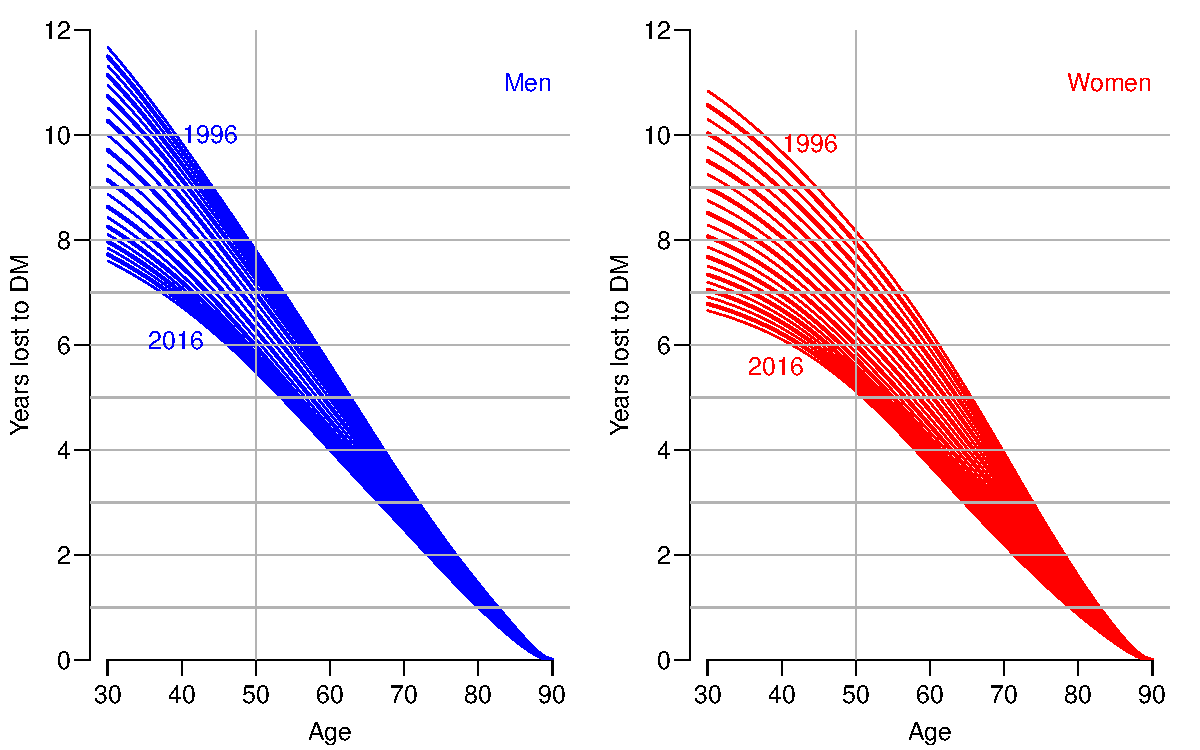
\includegraphics[width=\textwidth]{yll-imm}
  \caption{Years of life lost to DM: the difference in expected
    residual life time at different ages between persons with and
    without diabetes, assuming the persons without diabetes at a given
    age remain free from diabetes (immunity assumption --- not
    reasonable). The lines refer to date of evaluation; the top lines
    refer to 1.1.1996 the bottom ones to 1.1.2016. Blue curves are
    men, red women.}
  \label{fig:imm}
\end{figure}

\begin{figure}[h]
  \centering
  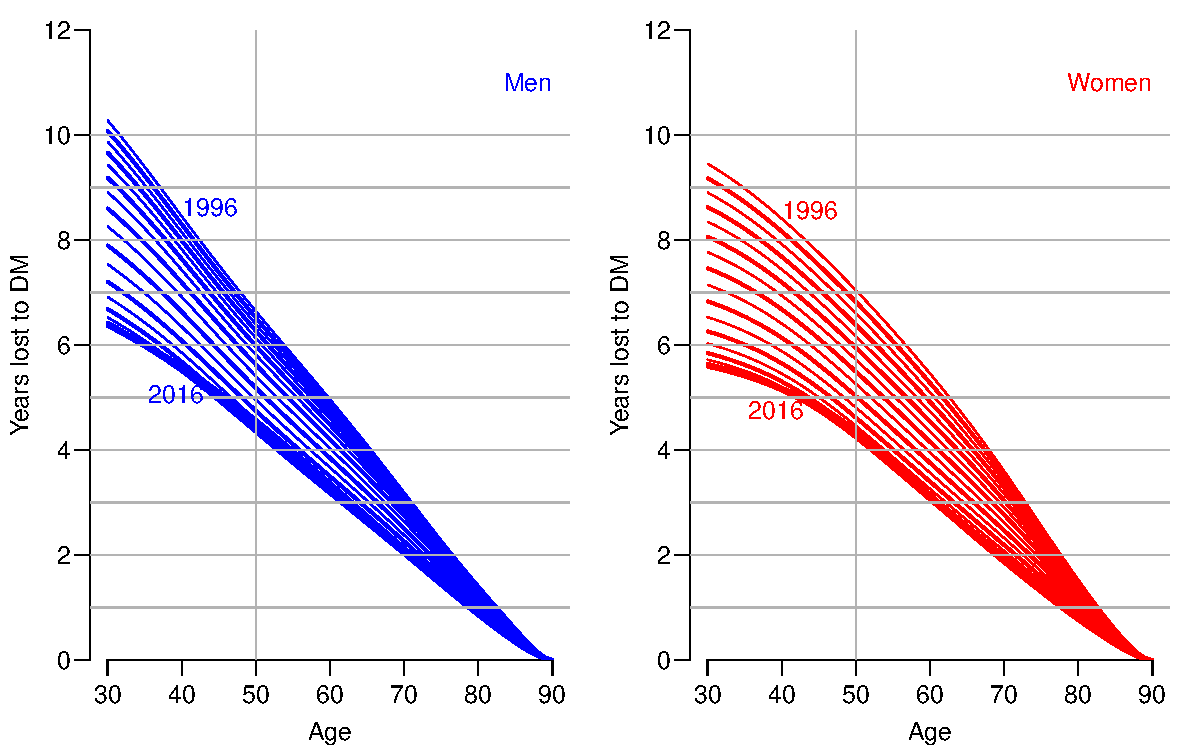
\includegraphics[width=\textwidth]{yll-sus}
  \caption{Years of life lost to DM: the difference in expected
    residual life time at different ages between persons with and
    without diabetes, allowing the persons without diabetes at a given
    to contract diabetes and thus be subject to higher mortality. The
    lines refer to date of evaluation; the top lines refer to 1.1.1996
    the bottom ones to 1.1.2016. Blue curves are men, red women.}
  \label{fig:sus}
\end{figure}

\begin{figure}[h]
  \centering
  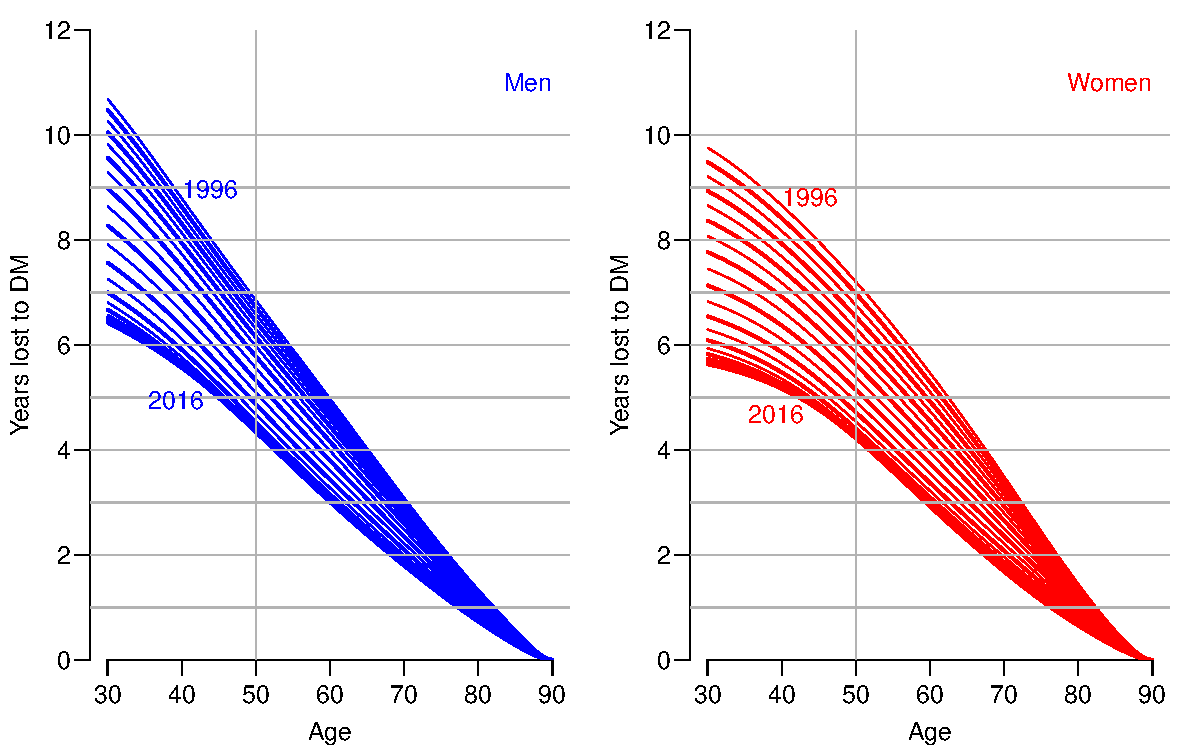
\includegraphics[width=\textwidth]{yll-tot}
  \caption{Years of life lost to DM: the difference in expected
    residual life time at different ages between persons with and
    without diabetes. Allowance for susceptibility is approximated by
    using the total population mortality instead of non-DM
    mortality. The lines refer to date of evaluation; the top lines
    refer to 1.1.1996 the bottom ones to 1.1.2016. Blue curves are
    men, red women.}
  \label{fig:tot}
\end{figure}

From figure \ref{fig:sus} we see that for men aged 50 the years lost to
diabetes has decreased from a bit over 8 to a bit less than 6 years,
and for women from 8.5 to 5 years; so a greater improvement for women.

\chapter{Practical implementation}

We have devised functions that wraps these formulae up for practical
use.

\section{Function definitions}

% The following code sources the originally formatted code in erl.R in
% order to make it printable with all the formatting and comments in
% it. However the sourcing does not work when compiling the vignettes
% in R CMD build. So when checking the code we comment this out by
% putting eval=FALSE. So depending on whether we actually construct
% the pdf for the inst/doc folder or test (upload) the package, one of
% the following two chunks are run with eval=FALSE and the other with
% eval=TRUE.
% When checking the package
When using the functions it is assumed that the functions $\mu_W$,
$\mu_D$ and $\lambda$ are given as vectors corresponding to
equidistantly (usually tightly) spaced ages from 0 to $K$ where K is
the age where everyone can safely be assumed dead.

\texttt{surv1} is a simple function that computes the survival
function from a vector of mortality rates, and optionally the
conditional survival given being alive at prespecified ages:
\begin{Schunk}
\begin{Sinput}
> surv1
\end{Sinput}
\begin{Soutput}
function (int, mu, age.in = 0, A = NULL) 
{
    if (any(is.na(mu))) {
        mu[is.na(mu)] <- 0
        warning("NAs in agument 'mu' set to 0")
    }
    age <- 0:length(mu) * int + age.in
    Mu <- c(0, cumsum(mu) * int)
    Sv <- exp(-Mu)
    surv <- data.frame(age = age, surv = Sv)
    if (cond <- !is.null(A)) {
        j <- 0
        cage <- NULL
        for (ia in A) {
            j <- j + 1
            cA <- which(diff(age > ia) == 1)
            surv <- cbind(surv, pmin(1, surv$surv/(surv$surv[cA])))
            cage[j] <- surv$age[cA]
        }
    }
    names(surv)[-1] <- paste("A", c(age.in, if (cond) cage else NULL), 
        sep = "")
    rownames(surv) <- NULL
    return(surv)
}
<bytecode: 0x8b1cd48>
<environment: namespace:Epi>
\end{Soutput}
\end{Schunk}
\texttt{erl1} basically just expands the result of \texttt{surv1} with
a column of expected residual life times:
\begin{Schunk}
\begin{Sinput}
> erl1
\end{Sinput}
\begin{Soutput}
function (int, mu, age.in = 0) 
{
    age <- 0:length(mu) * int + age.in
    musmuc <- function(x) rev(cumsum(rev(x)))
    surv <- surv1(int = int, mu = mu, age.in = age.in)[, 2]
    cbind(age = age, surv = surv, erl = c(musmuc((surv[-1] - 
        diff(surv)/2))/surv[-length(surv)], 0) * int)
}
<bytecode: 0x84c6e48>
<environment: namespace:Epi>
\end{Soutput}
\end{Schunk}
We also define a function, \texttt{surv2}, that computes the survival
function for a non-diseased person that may become diseased with rate
\texttt{lam} and after that die at a rate of \texttt{muD}
(corresponding to the formulae above). This is the sane way of
handling years of life lost to a particular illness:
\begin{Schunk}
\begin{Sinput}
> surv2
\end{Sinput}
\begin{Soutput}
function (int, muW, muD, lam, age.in = 0, A = NULL) 
{
    if (length(muW) != length(muD) | length(muD) != length(lam)) 
        stop("Vectors with rates must have same length:\n", "length(muW)=", 
            length(muW), ", length(muD)=", length(muD), ", length(lam)=", 
            length(lam))
    if (!is.null(lam)) {
        if (any(is.na(lam))) {
            lam[is.na(lam)] <- 0
            warning("NAs in agument 'lam' set to 0")
        }
    }
    if (any(is.na(muD))) {
        muD[is.na(muD)] <- 0
        warning("NAs in agument 'muD' set to 0")
    }
    if (any(is.na(muW))) {
        muW[is.na(muW)] <- 0
        warning("NAs in agument 'muW' set to 0")
    }
    wsurv2 <- function(int, muW, muD, lam, age.in = 0, A = 0) {
        age <- 0:length(muW) * int + age.in
        MuW <- cumsum(c(0, muW) * (age > A)) * int
        MuD <- cumsum(c(0, muD) * (age > A)) * int
        Lam <- cumsum(c(0, lam) * (age > A)) * int
        pW <- exp(-(Lam + MuW))
        Dis <- c(0, lam) * (age > A) * exp(-(Lam + MuW)) * int
        pDM <- Dis * 0
        for (ia in 1:length(age)) pDM[ia] <- sum(Dis[1:ia] * 
            exp(-(MuD[ia] - MuD[1:ia])))
        surv <- data.frame(age = age, surv = pDM + pW)
        return(surv)
    }
    surv <- wsurv2(int, muW, muD, lam, age.in = age.in, A = 0)
    if (!is.null(A)) {
        for (j in 1:length(A)) {
            surv <- cbind(surv, wsurv2(int, muW, muD, lam, age.in = age.in, 
                A = A[j])[, 2])
        }
    }
    Al <- A
    for (i in 1:length(A)) Al[i] <- max(surv$age[surv$age <= 
        A[i]])
    colnames(surv)[-1] <- paste("A", c(age.in, Al), sep = "")
    return(surv)
}
<bytecode: 0x851ba70>
<environment: namespace:Epi>
\end{Soutput}
\end{Schunk}
Finally we devised a function using these to compute the expected
residual lifetime at select ages:
\begin{Schunk}
\begin{Sinput}
> erl
\end{Sinput}
\begin{Soutput}
function (int, muW, muD, lam = NULL, age.in = 0, A = NULL, immune = is.null(lam), 
    yll = TRUE, note = TRUE) 
{
    trsum <- function(x) {
        x[c(diff(x) == 0, TRUE)] <- NA
        sum((x[-length(x)] + x[-1])/2, na.rm = TRUE)
    }
    if (!immune & is.null(lam)) 
        stop("'lam' is required when immune=FALSE\n")
    if (!is.null(lam)) {
        if (any(is.na(lam))) {
            lam[is.na(lam)] <- 0
            warning("NAs in agument 'lam' set to 0")
        }
    }
    if (any(is.na(muD))) {
        muD[is.na(muD)] <- 0
        warning("NAs in agument 'muD' set to 0")
    }
    if (any(is.na(muW))) {
        muW[is.na(muW)] <- 0
        warning("NAs in agument 'muW' set to 0")
    }
    sD <- surv1(int = int, muD, age.in = age.in, A = A)
    if (immune) 
        sW <- surv1(int = int, muW, age.in = age.in, A = A)
    else sW <- surv2(int = int, muW, muD, lam, age.in = age.in, 
        A = A)
    erl <- cbind(apply(sW[, -1], 2, trsum), apply(sD[, -1], 2, 
        trsum)) * int
    colnames(erl) <- c("Well", "Dis")
    rownames(erl) <- colnames(sW)[-1]
    if (yll) 
        erl <- cbind(erl, YLL = erl[, "Well"] - erl[, "Dis"])
    if (immune) {
        attr(erl, "NOTE") <- "Calculations assume that Well persons cannot get Ill (quite silly!)."
        if (note) 
            cat("NOTE:", attr(erl, "NOTE"), "\n")
    }
    return(erl)
}
<bytecode: 0x8b43728>
<environment: namespace:Epi>
\end{Soutput}
\end{Schunk}
\ldots and a wrapper for this if we only want the years of life lost
returned:
\begin{Schunk}
\begin{Sinput}
> yll
\end{Sinput}
\begin{Soutput}
function (int, muW, muD, lam = NULL, age.in = 0, A = NULL, immune = is.null(lam), 
    note = TRUE) 
erl(int = int, muW = muW, muD = muD, lam = lam, age.in = age.in, 
    A = A, immune = immune, yll = TRUE, note = note)[, "YLL"]
<bytecode: 0xa8a8c00>
<environment: namespace:Epi>
\end{Soutput}
\end{Schunk}

\bibliographystyle{plain}

\begin{thebibliography}{1}

\bibitem{Carstensen.2007a}
B~Carstensen.
\newblock Age-{P}eriod-{C}ohort models for the {L}exis diagram.
\newblock {\em Statistics in Medicine}, 26(15):3018--3045, 2007.

\bibitem{Carstensen.2008c}
B~Carstensen, JK~Kristensen, P~Ottosen, and K~Borch-Johnsen.
\newblock The {D}anish {N}ational {D}iabetes {R}egister: {T}rends in incidence,
  prevalence and mortality.
\newblock {\em Diabetologia}, 51:2187--2196, 2008.

\end{thebibliography}

\addcontentsline{toc}{chapter}{References}

\end{document}
